\section{Data analysis and Validation}

\graphicspath{{Chapter3/Figs/}}

\begin{frame}[t]
  \frametitle{Input Datasets}
  \framesubtitle{}
  \label{ch3:data}
  
  \textbf{For validation:}
  \begin{enumerate}
    \item EPN network, solution C2010 - ETRF 2014 (299 stations)
    \item EPOS network, INGV solution (571 stations)
    \item \textbf{EPOS network, CNRS solution (MIDAS) (452 stations)}
    \item network GREECE, NTUA reprocessing 2017 (153 stations)
  \end{enumerate}
  \vskip .4cm
  \textbf{Softwares used for validation:}
  \begin{enumerate}[(I)]
    \item \textbf{VISR:} free, Linux-based, needs own scripting of plotting tools \citep{Shen1996}
    \item \textbf{STIB:} needs request, python-based, Spakman \& Nyst method
    
    \citep{Masson2014}
    \item \textbf{SSPX:} free, Mac-based, VISR method \citep{Cardozo2008}
  \end{enumerate}
  
%   VISR/VISR2 (Shen et al. 1996, JGR; 2015, BSSA), free, 2D and 3D
% strain, Linux-based, needs own scripting of plotting tools
% 
% STIB (Masson et al. 2014, GJI), needs request, python-based,
% Spakman & Nyst method (SNM)
% 
% SSPX (Cardoso & Allmendinger 2009, Comp. Geosci.), free, 2D and
% 3D strain, Mac-based, VISR method

  In this study we present results using CNRS (MIDAS). 
    
\end{frame}
\note{}

\begin{frame}[t]
  \frametitle{Validation}
  \framesubtitle{$e_{max}$ - $e_{min}$ maps comparison}
  \label{ch3:data}
%   \textcolor{red}{TODO: datasets}
  \begin{columns}
    \begin{column}{0.5\textwidth}
      \begin{center}
        \textbf{VISR} 
        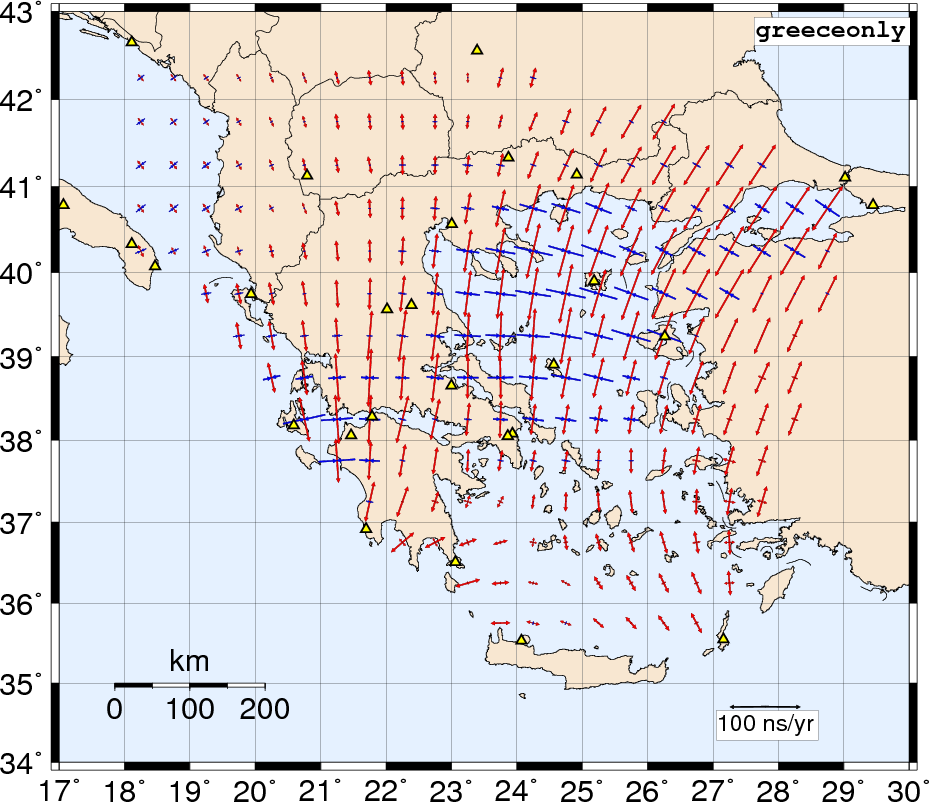
\includegraphics[width=.98\textwidth]{a1_map_strain_vectors.png}   
      \end{center}
    \end{column}
    \begin{column}{0.5\textwidth}
      \begin{center}
        \textbf{PyStrain} 
        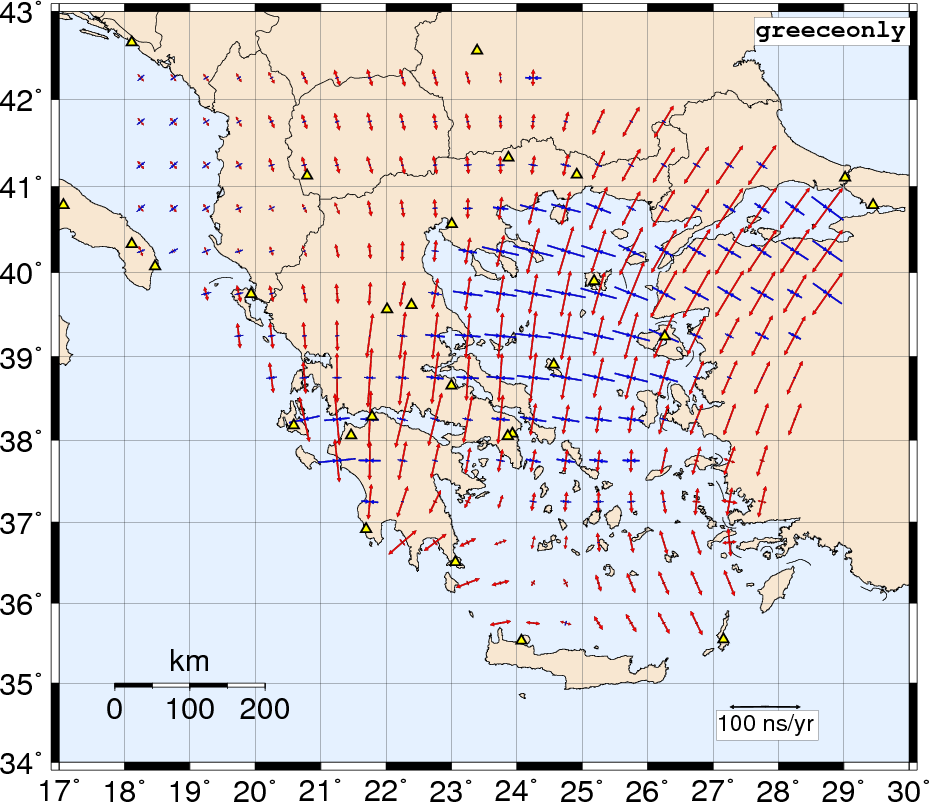
\includegraphics[width=0.98\textwidth]{a2_map_strain_vectors.png}     
      \end{center}
    \end{column}
  \end{columns}

\end{frame}
\note{}

% \begin{frame}
%   \frametitle{Validation}
%   \framesubtitle{dilatation maps comparison}
%   \label{ch3:data}
%   \textcolor{red}{maybe a wrong dataset}
%   \begin{columns}
%     \begin{column}{0.5\textwidth}
%       VISR
%       
%       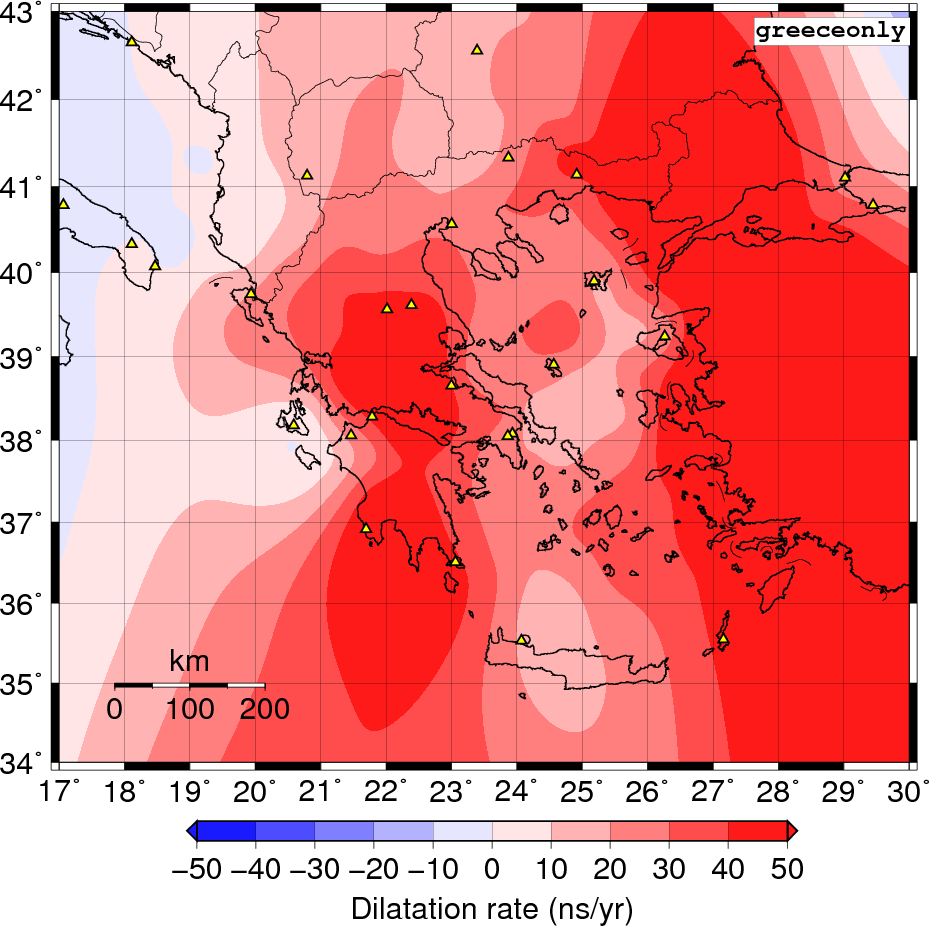
\includegraphics[width=.9\textwidth]{b1_map_strain_dilatation.png}   
%     \end{column}
%     \begin{column}{0.5\textwidth}
%     \begin{center}
%       PyStrain
%       
%       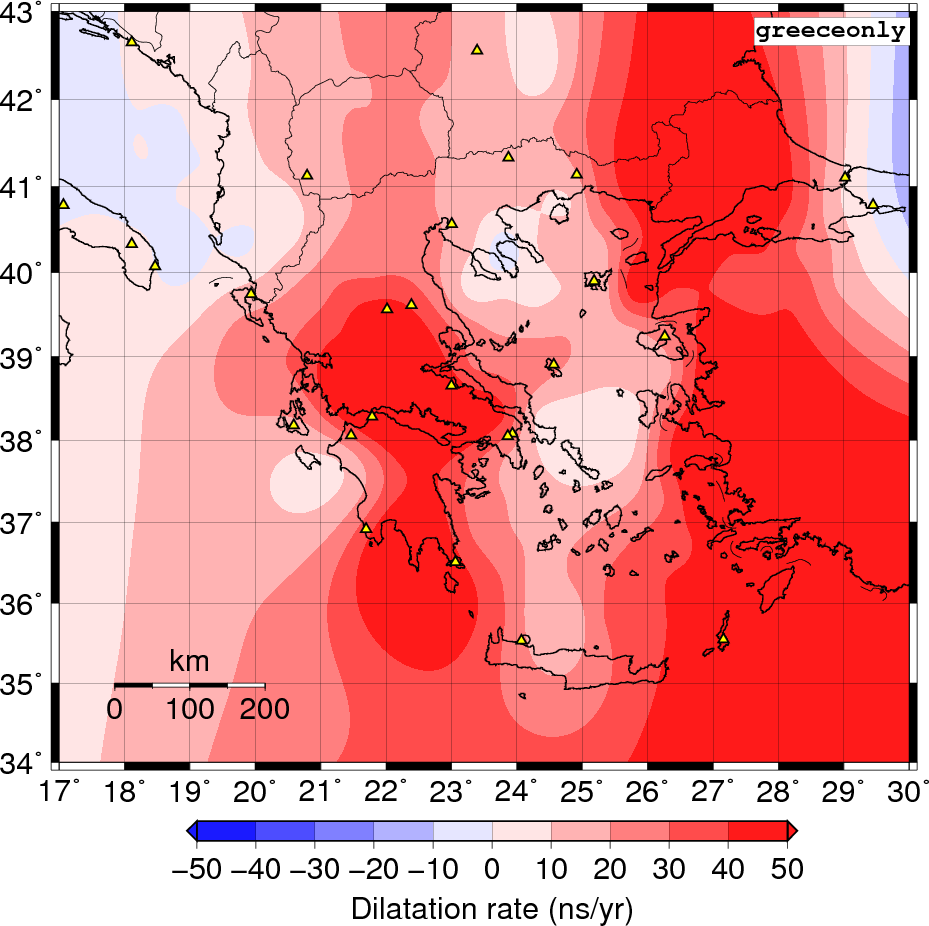
\includegraphics[width=0.9\textwidth]{b2_map_strain_dilatation.png}     
%     \end{center}
%     \end{column}
%   \end{columns}
% 
% \end{frame}
% \note{}

\begin{frame}
  \frametitle{Validation}
  \framesubtitle{differences}
  \label{ch3:data}
  \vskip-.5cm
  \begin{columns}
    \begin{column}{0.5\textwidth}
      \begin{center}
        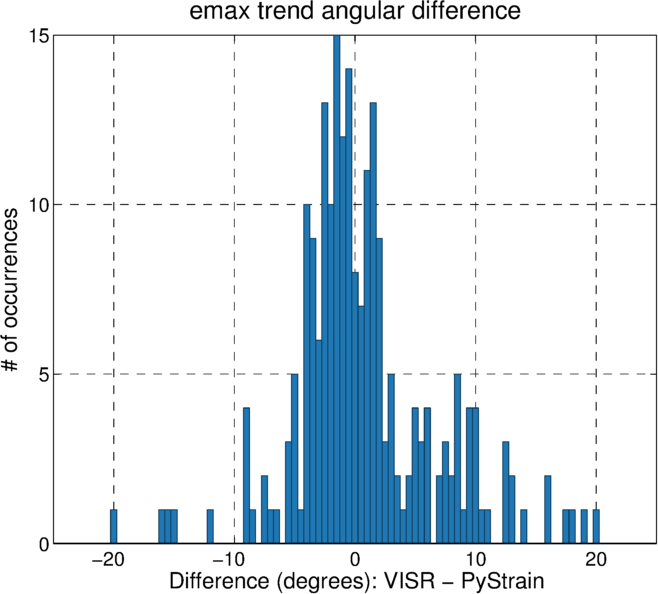
\includegraphics[width=.71\textwidth]{diff-emax-trend_VISR-vs-PyStrain.png}
        \vskip .2cm
        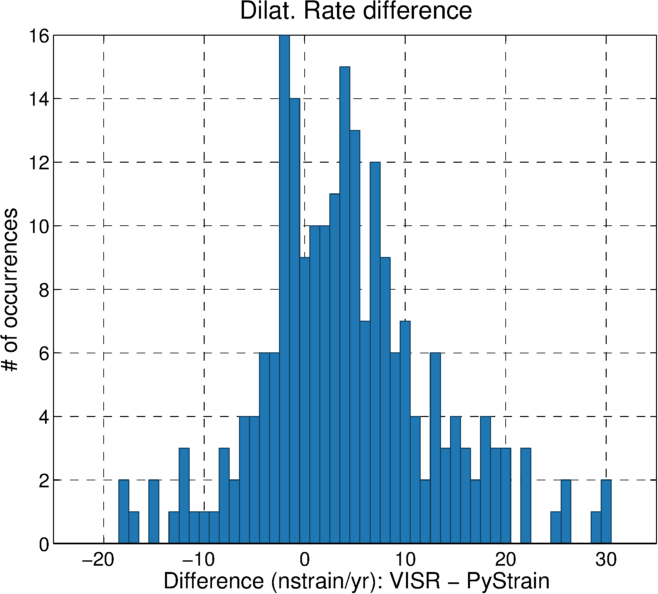
\includegraphics[width=.71\textwidth]{diff-dilat_VISR-vs-PyStrain.png}
      \end{center}
    \end{column}
    \begin{column}{0.5\textwidth}
      \begin{center}
        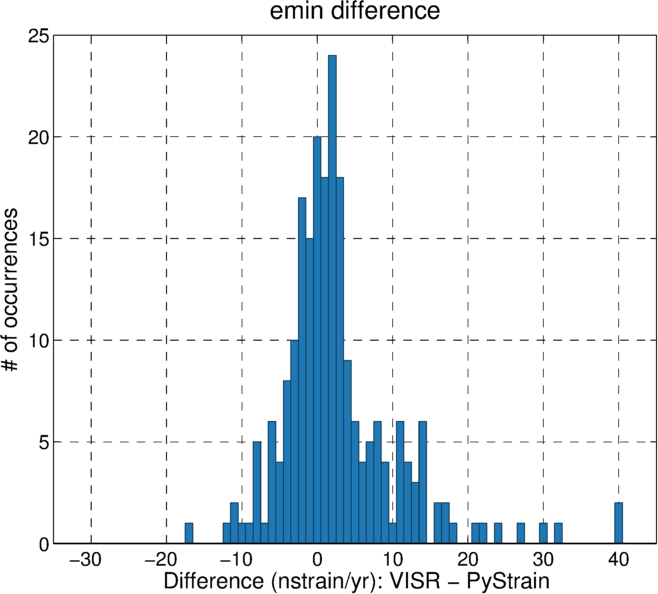
\includegraphics[width=.71\textwidth]{diff-emin_VISR-vs-PyStrain.png}
        \vskip .2cm
        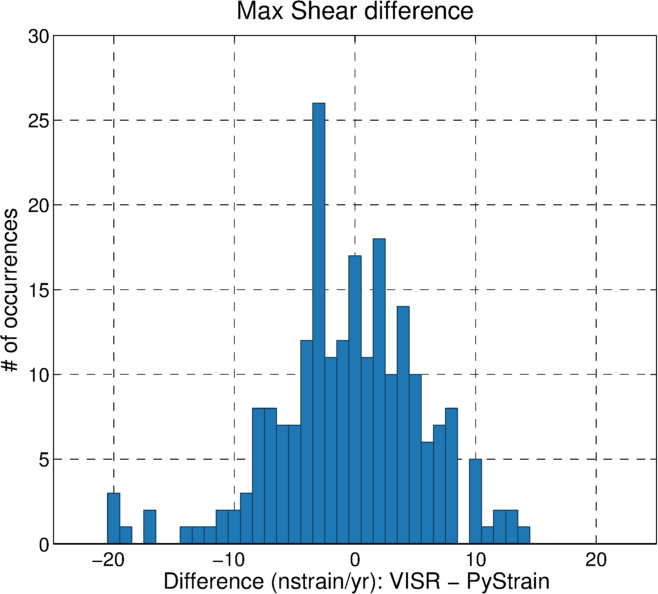
\includegraphics[width=.71\textwidth]{diff-shear_VISR-vs-PyStrain.png}     
      \end{center}
    \end{column}
  \end{columns}

\end{frame}
\note{}

\begin{frame}
  \frametitle{Validation}
  \framesubtitle{histograms}
  \label{ch3:data}
  \vskip-.5cm
  \begin{columns}
    \begin{column}{0.5\textwidth}
      \begin{center}
        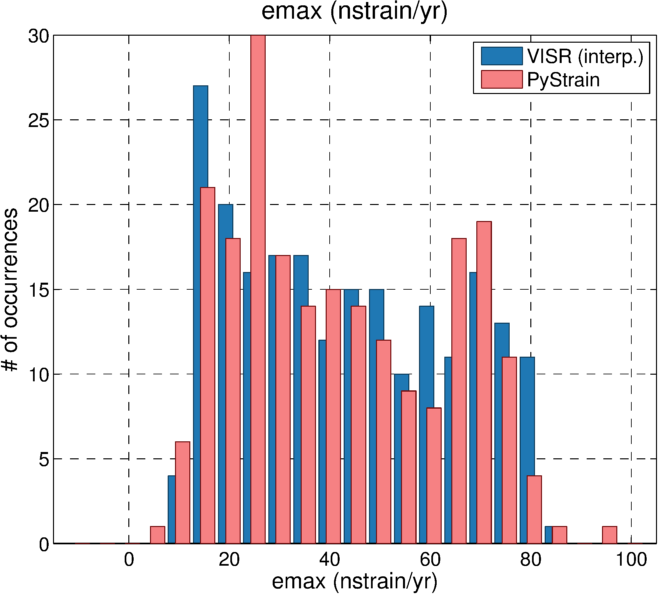
\includegraphics[width=.71\textwidth]{emax_hist_VISR-vs-PyStrain.png}
        \vskip .15cm
        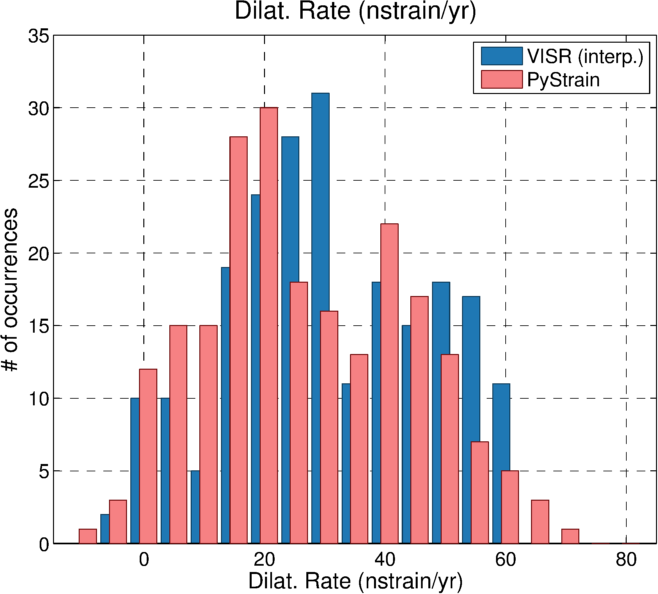
\includegraphics[width=.71\textwidth]{dilat_hist_VISR-vs-PyStrain.png}
      \end{center}
    \end{column}
    \begin{column}{0.5\textwidth}
      \begin{center}
        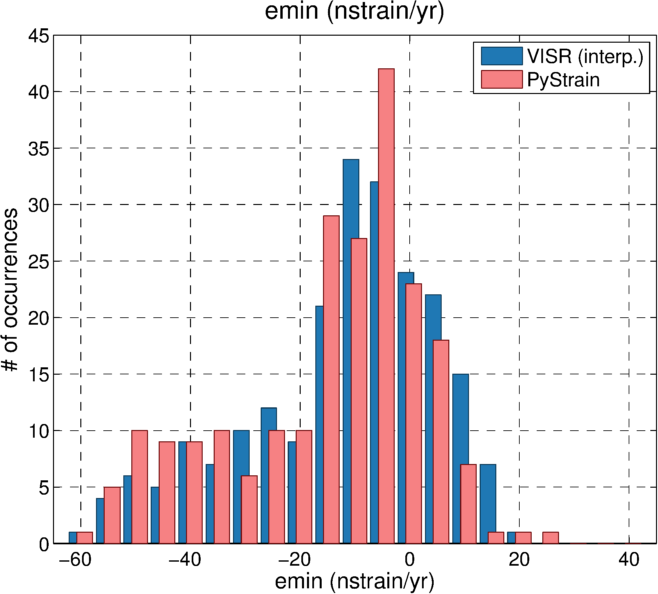
\includegraphics[width=.71\textwidth]{emin_hist_VISR-vs-PyStrain.png}
        \vskip .15cm
        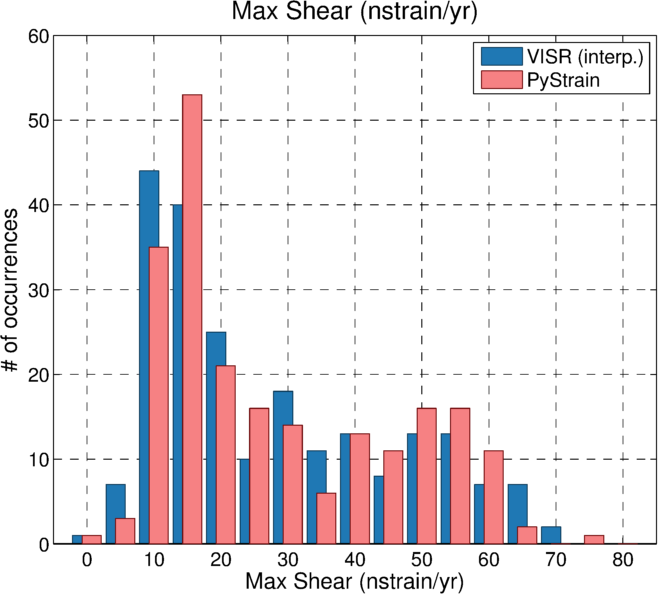
\includegraphics[width=.71\textwidth]{shear_hist_VISR-vs-PyStrain.png}     
      \end{center}
    \end{column}
  \end{columns}

\end{frame}
\note{}


%\begin{frame}
%  \frametitle{Συμπεράσματα}
%  \framesubtitle{}
%  \label{ch3:}

%\end{frame}
%\note{}
